\documentclass{article}
\usepackage[colorlinks=true]{hyperref}
\usepackage{geometry}
\usepackage{fancyhdr}
\usepackage{palatino}
\usepackage{titlesec}
\usepackage{pbox}
\usepackage{multicol}
\usepackage{graphicx}
\usepackage{amsmath}
\usepackage{enumitem}

\renewcommand{\baselinestretch}{1.15}
\geometry{margin=1in}
\geometry{headheight=2in}
\geometry{top=2in}
\titlespacing\section{0pt}{12pt plus 2pt minus 2pt}{0pt plus 2pt minus 2pt}
\lhead{}
\rhead{}
\pagestyle{fancy}
\setlength{\parskip}{0.5em}
\date{\today}

\title{CS 145 Milestone 3 - ToMEto}
\author{Jonathan Joo, Matthew Jin, Boyu (Charlie) Tong, Albert Ge}
\chead{%
  {\vbox{%
      \vspace{2mm}
      \large
      Networks: Structure Economics \hfill
      Caltech CMS/CS/EE 145 \hfill \\[1pt]
      CS 145 Milestone 3 - ToMEto \hfill
      \date{\today} \\
    }
  }
}



\begin{document}
\maketitle
\section{Goals}
This week, we wanted to accomplish
\begin{enumerate}
% \setlength{\itemsep}{0em}
    \item Implement (more) algorithms
    \item Improve data quality
    \item Integration of frontend with backend
\end{enumerate}



\section{Progress}
Our project now has all the basic components completed and integrated together. We have completed all the goals for these two weeks, and now have a working prototype for our basic use case!


\subsection{Implement (more) algorithms}
We have implemented/tested several algorithms at this point, and can easily switch between them when starting up the website. We have not yet determined a ``best'' algorithm, and are still trying out more ideas:
\begin{itemize}
% \setlength{\itemsep}{0em}
  \item (DONE) Naive, degree-based
  \item (DONE) Pairwise PMI
  \item Generalized PMI
  \item PMI with minimax or other constraints
\end{itemize}


\subsection{Improve data quality}
We implemented an ingredient preprocessor that maps ``low quality'' or ``noisy'' ingredients to better ingredients. The goal is to limit the set of ingredients and get a better representation of the actual components for each recipe. For example, some mappings are:
\begin{itemize}
% \setlength{\itemsep}{0em}
  \item medium-large shrimps (about 14 to 16) $\to$ shrimps
  \item slices freshly toasted french bread $\to$ french bread
  \item small potatoes, cooked, peeled and sliced $\to$ potatoes
\end{itemize}


\subsection{Integration of frontend with backend}
The website is now fully functional for our basic use case. There is a tab where the user can input search queries for recipes. The queries are forwarded to the backend, where it is processed into relevant recipe results. For each recipe returned, the frontend can display the recommended ingredients to add.
\begin{center}

\includegraphics[scale=0.4]{M3_img1.png}
$\quad\quad$
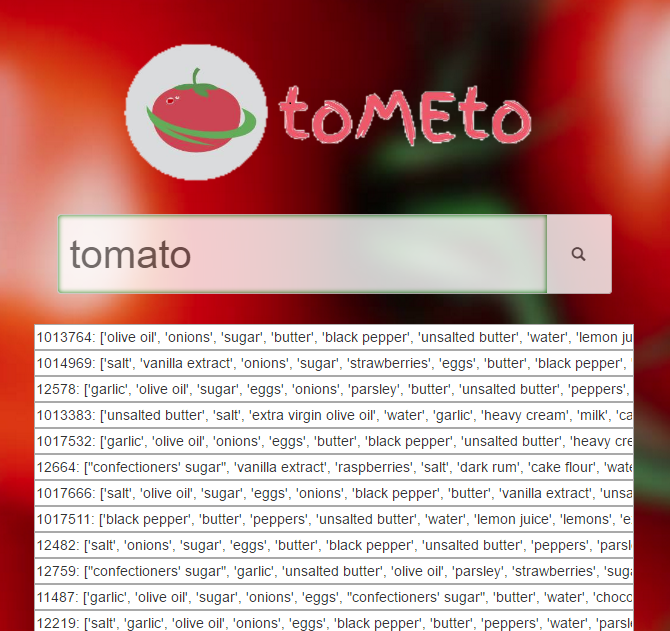
\includegraphics[scale=0.4]{M3_img2.png}
\end{center}
We currently forward the search query to the actual NYT website and use their search results. We thought this was the simplest and best way to handle the queries without having to develop our own search engine.


\subsection{Design improvements}
We also refactored our codebase in order to make the entire flow of the program much easier to picture and understand. There are now distinct components for everything that we do, modularized in a logical way which allows for easy modification, testing, and integration:
\begin{itemize}
% \setlength{\itemsep}{0em}
  \item Data scraper + parser: \texttt{scraper.py, parser.py}
  \item Ingredient preprocessor: \texttt{mapper.py}
  \item Ingredient recommender: \texttt{analyzer\_*.py}
  \item Frontend: \texttt{app.py}
\end{itemize}



\section{Contributions}
\textbf{Jonathan Joo:} Worked on integrating backend with frontend via search.

\textbf{Matthew Jin:} Worked on backend of search and mapper, and researched Amazon Mechanical Turk.

\textbf{Charlie Tong:} Worked on \texttt{mapper.py}, code refactoring, and frontend/backend integration.

\textbf{Albert Ge:} Worked on more algorithms (generalized PMI, PMI with constraints).



\section{Adjustments to plan}

We have improved our results since the last milestone by improving data quality and minor adjustments to our algorithms. On the backend, we will probably try more algorithms and ideas. This includes expanding on our current implementations (naive, PMI) by trying different variants. We will also do some more research and see if there are other techniques that we can utilize.

On the frontend, the GUI and interface are functional at the basic level. We will continue to improve the integration and include more features. Right now the data is presented as a list, which is clearly not optimal for the user. We will make the search results more presentable and have an actual landing page for each recipe. This will be in line with our fourth milestone goal to ``Complete GUI front-end''.

\end{document}
